%=================================================================
%\section{Unsupervised expansion of ad-hoc abbreviations in EHR narratives}
\section{Materials and Methods}

%-----------------------------------------------------------------
%\subsection{Materials and Methods}

\begin{frame}
	\frametitle{Materials and Methods}
	\begin{itemize} \myspacing
		\item 30,000 clinical documents from the cardiology domain
		\begin{itemize}
			\item Written in German by Austrian physicians
			\item Discharge summaries, finding reports        
                         \item Routine documentation in LKH, Graz
                \end{itemize}

	\end{itemize}
\end{frame}

\begin{frame}
	\frametitle{Materials and Methods}
                \begin{figure}
        			\centering
        			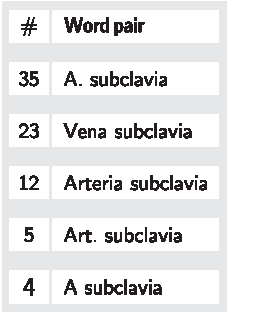
\includegraphics[height=5cm]{bigram.pdf}
        			\caption{Building a bigram (word pair) list.}
        			\label{fig:bigram_extraction}
  		\end{figure}
\end{frame}

\begin{frame}
	\frametitle{Materials and Methods}
                \begin{figure}
        			\centering
        			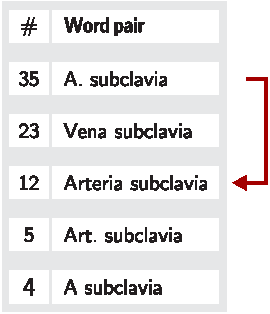
\includegraphics[height=5cm]{bigram_lookup.pdf}
        			\caption{Lookup in a bigram (word pair) list.}
        			\label{fig:bigram_lookup}
  		\end{figure}
\end{frame}

\begin{frame}
	\frametitle{Materials and Methods}
	\begin{itemize} \myspacing
	        \item Evaluation data
                \begin{itemize}
                		\item 200 random text excerpts centered on an abbreviation
			\item 147 abbreviations manually expanded by a human annotator
                \end{itemize}
%                \item ``Big data'': extract knowledge from available data
%                \begin{itemize}
%	                \item Unsupervised machine learning
%	                \item Training-test split (90\% - 10\%)
%		        \item Bigram (word pair) list lookup
%                \end{itemize}
	        \item Evaluation method
                \begin{itemize}
                		\item Recall (R): sensitivity
			\item Precision (P): positive predictive value
			\item $F$-score ($F_1$): harmonic mean of precision and recall
                \end{itemize}
	\end{itemize}
\end{frame}

%-----------------------------------------------------------------


